\section{Regularization}



% -----------------------------------------------------------------------------
\begin{frame}\frametitle{Regularization}
	\begin{block}{Risk function}
		\begin{equation*}
			R_{[\vec{w}]} = \underbrace{ E_{[\vec{w}]}^T }_{
					\substack{\text{training} \\ \text{error}}}
				+ \underbrace{ \lambda E_{[\vec{w}]}^R }_{
					\substack{\text{regularization} \\ \text{term}}}
				\eqexcl \min 
		\end{equation*}
		\begin{itemize}
			\item $E^R:$ prior knowledge of solution
			\item $\lambda:$ regularization parameter 
		\end{itemize}
	\end{block}
	
	\begin{center}
		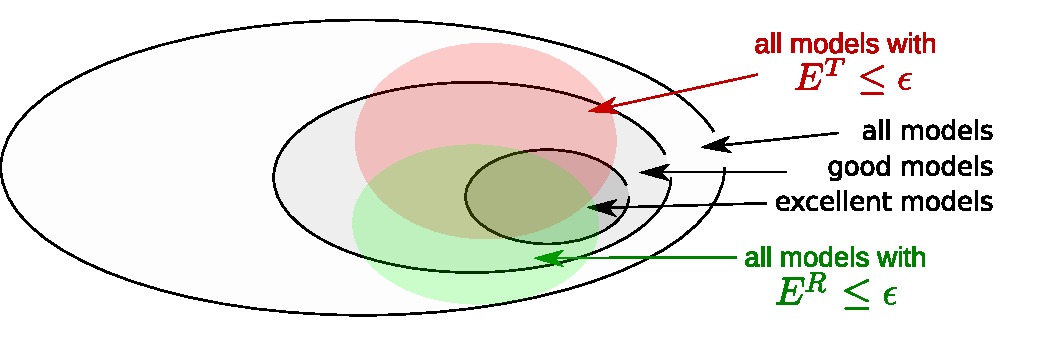
\includegraphics[width=10cm]{img/ModelSelection_models_v2.pdf}
	\end{center}
\end{frame}


% -----------------------------------------------------------------------------
\begin{frame}\frametitle{Regularization example: weight decay}
	\begin{equation*}
		E_{[\vec{w}]}^R \quad=\quad \frac{1}{2} \sum_{(i, j, v', v)} 
			\big( \mathrm{w}_{ij}^{v'v} \big)^2
	\end{equation*}
	%\vspace{2mm}
	
	\begin{center}
		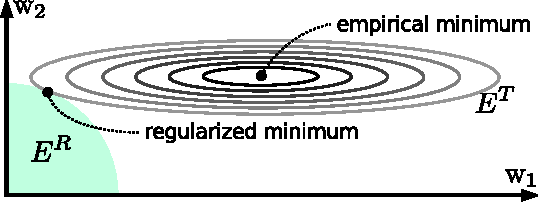
\includegraphics[width=7cm]{img/empirical_vs_regularized}
	\end{center}

	%\vspace{2mm}
	\begin{block}{Minimization of $R$ through gradient descent}
		\begin{equation*}
			\Delta \mathrm{w}_{ij}^{v'v} \quad\sim\quad 
				-\frac{\partial R}{\partial \mathrm{w}_{ij}^{v'v}}
			\quad=\quad - \underbrace{\frac{\partial E^T}%
				{\partial \mathrm{w}_{ij}^{v'v}}}_{
				\substack{\text{e.g. via} \\ \text{backprop}}}
			\;\;-\;\; \underbrace{\lambda \mathrm{w}_{ij}^{v'v}}_{
				\substack{\text{decay} \\ \text{term}}}
		\end{equation*}
	\end{block}
\end{frame}


% -----------------------------------------------------------------------------
\begin{frame}\frametitle{Other forms of regularization}
	\iitem{ general form of regularization: 
		$E^R = \sum\limits_{(i, j, v', v)} {|w_{ij}^{v'v}|}^q$}
	\begin{center}
		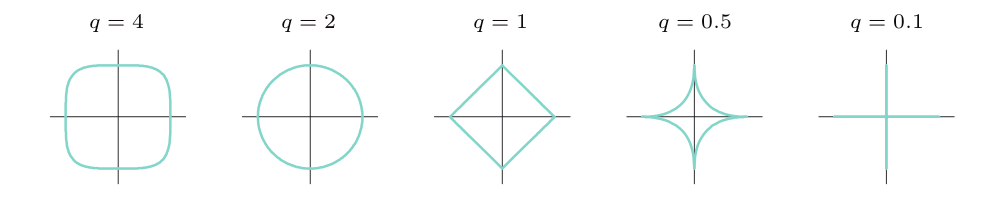
\includegraphics[width=9.5cm]{img/QnormPenalties_clean.png} \\
		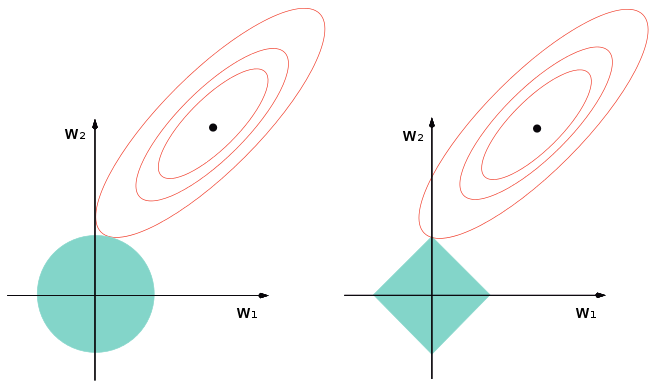
\includegraphics[width=7cm]{img/RegularizationTypesIntersect_clean.png} \\[-2mm]
		{ \footnotesize $L_2$ {\em weight decay} with $q=2$ 
			\hspace{1cm} $L_1$ {\em lasso} with $q=1$ \hspace{1cm} $ $}
	\end{center}

\end{frame}


% -----------------------------------------------------------------------------
\begin{frame}\frametitle{Regularization example: symmetries} 
	Odd vs. even function
	\begin{equation*}
		E_{[\mathrm{w}]}^R = \frac{1}{2p} \sum_{\alpha = 1}^p 
			\Big( y_{(\vec{x}^{(\alpha)}; \vec{w})} 
				\pm y_{(-\vec{x}^{(\alpha)}; \vec{w})} 
			\Big)^2
	\end{equation*}
	\pause
	Invariance under translation:
	\begin{equation*}
		E_{[\mathrm{w}]}^R = \frac{1}{2p} \sum_{\alpha = 1}^p 
			\Big( y_{(\vec{x}^{(\alpha)}; \vec{w})} 
				- y_{(\vec{x}^{(\alpha)} - \vec{t}; \vec{w})} 
			\Big)^2
	\end{equation*}
	\pause
	Monotony:
	\begin{equation*}
		E_{[\mathrm{w}]}^R = \frac{1}{n_p} \sum_{
			\mathrm{x}^{(\alpha)} > \mathrm{x}^{(\beta)}} 
		\left \{
		\begin{array}{cl}
			\Big( y_{(\vec{x}^{(\alpha)}; \vec{w})} - 
				y_{(\vec{x}^{(\beta)}; \vec{w})} \Big)^2  
			& \text{if } y_{(\vec{x}^{(\alpha)}; \vec{w})} < 
				y_{(\vec{x}^{(\beta)}; \vec{w})} \\[2mm] 
			0 & \text{else}
		\end{array} \right.
	\end{equation*}
\end{frame}

% ------------------------------------------------------------------------------
\begin{frame} \frametitle{Early stopping}
	\begin{center}
		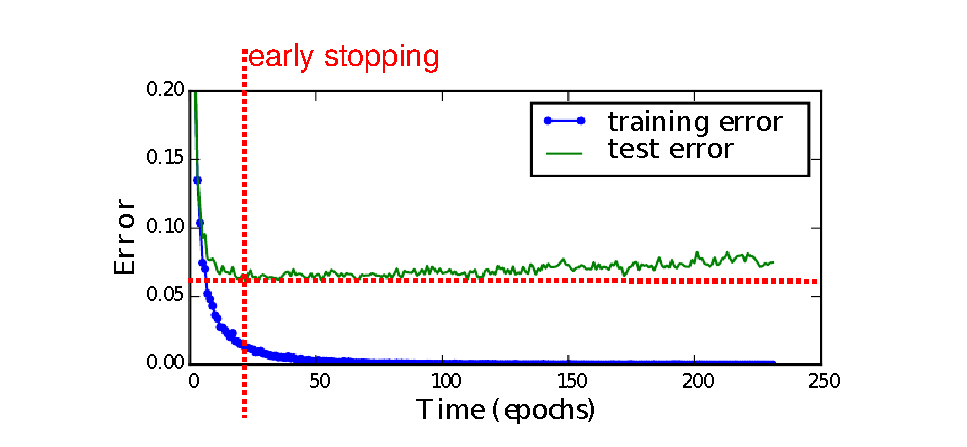
\includegraphics[width=10cm]{img/early_stopping.pdf}
	\end{center}
	\iitem{Estimate generalization error with a test set during training.}
	\iitem{Stop training when the error on the test set rises.}
	\blfootnote{\hfill (trained on MNIST, Goodfellow et al., 2016)}
\end{frame}

% ------------------------------------------------------------------------------


% -----------------------------------------------------------------------------
\begin{frame}\frametitle{Choice of regularization parameter}
	\begin{block}{Testset method}
		\begin{enumerate}
		  \item perform model selection for different values of $\lambda$\\ 
		  		(on training data) 
		  \item<2-> select value of $\lambda$, 
		  		which provides best prediction results\\ 
				(on test data) 
		  \item<3-> estimate generalization performance of selected $\lambda$\\
		  		(on validation data)
		\end{enumerate}
	\end{block}	
	
	\vspace{1cm} 
	
	$ $\hspace{1cm}
	\includegraphics<1->[width=8cm]{img/traintestvalidation.pdf} 
\end{frame}


% -----------------------------------------------------------------------------
\begin{frame}\frametitle{Choice of regularization parameter}
	\begin{block}{$n$-fold cross-validation}
		\For{$\lambda = \lambda_1$ {\em\textbf{to}} $\lambda_n$}{
			perform $n$-fold cross-validation on 
				data with regularization $\lambda$
		}
		\vspace{2mm}

		pick optimal $\lambda^{\text{opt}}$ with minimum $\widehat{E}^G$\\
		\vspace{2mm}

		\textbf{final model:} train network on all data with $\lambda^{\text{opt}}$ 
	\end{block}
	
	\vspace{2mm}
	\begin{center}
		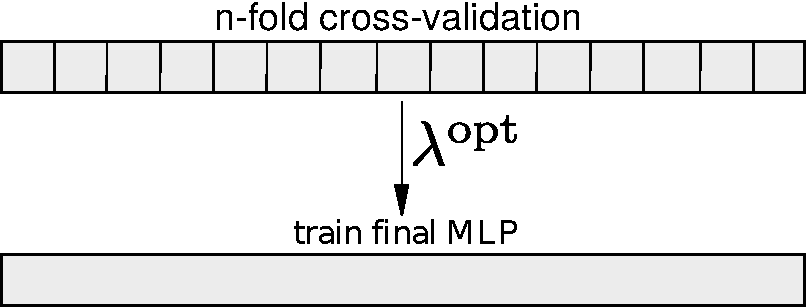
\includegraphics[width=8cm]{img/nfoldcrossvalidation.pdf} 
	\end{center}
\end{frame}


% -----------------------------------------------------------------------------
\begin{frame}\frametitle{Validation}
	\begin{itemize}
	\item[\textcircled{1}]
	$ \begin{array}{ll}
		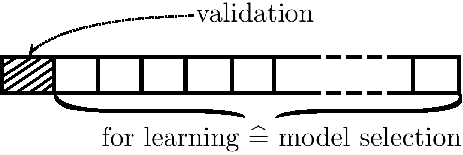
\includegraphics[height=1.2cm]{img/section1_fig34}
		& \begin{array}{ll}
			\bullet & \text{\footnotesize do n - 1 
				cross-validation for all values of } \lambda \\
			\bullet & \text{\footnotesize train with best $\lambda$} \\
			\bullet & \text{\footnotesize validate with learned model}
		\end{array}
	\end{array} $
	%\pause
	\item[\textcircled{2}]
	$ \begin{array}{ll}
		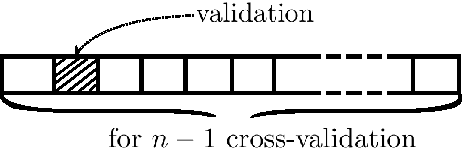
\includegraphics[height=1.2cm]{img/section1_fig35}
		& \begin{array}{ll}
			\bullet & \text{\footnotesize do n - 1 
				cross-validation for all values of } \lambda \\
			\bullet & \text{\footnotesize train with best $\lambda$} \\
			\bullet & \text{\footnotesize validate with learned model}
		\end{array}
	\end{array} $
	%\pause
	\item[\textcircled{n}]
	$ \begin{array}{ll}
		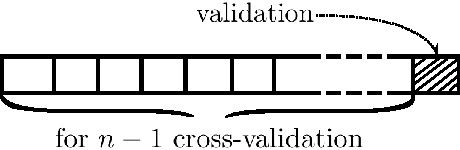
\includegraphics[height=1.2cm]{img/section1_fig36}
		& \begin{array}{ll}
			\bullet & \text{\footnotesize do n - 1
				cross-validation for all values of } \lambda \\
			\bullet & \text{\footnotesize train with best $\lambda$} \\
			\bullet & \text{\footnotesize validate with learned model}
		\end{array}
	\end{array} $
	\end{itemize}
	
	\begin{itemize}
		\item $\widehat{E}^G \quad\corresponds\quad$ 
			average over all $n$ validation errors
	\end{itemize}
\end{frame}


% -----------------------------------------------------------------------------
\begin{frame} 
	\begin{itemize}
		\item Never use test data for model selection 
			(including hyper-parameter search).
		\vspace{4mm}
		\item Always embed the whole selection procedure (including 
			hyper-parameter search) within an $n$-fold cross-validation run.
	\end{itemize}
\end{frame}

